\documentclass[a4paper, 12pt]{article}

\usepackage{geometry}
\geometry{left=2cm, right=2cm, top=2cm, bottom=2cm}

\usepackage{cmap}
\usepackage{mathtext} 
\usepackage[T2A]{fontenc}
\usepackage[utf8]{inputenc}
\usepackage[english,russian]{babel}	

\usepackage{amsfonts,amssymb,amsthm,mathtools}
\usepackage{amsmath}
\usepackage{icomma} 

\usepackage{graphicx} 
\graphicspath{{picturies/}}
\usepackage{wrapfig}

\usepackage{array,tabularx,tabulary,booktabs}
\usepackage{longtable}
\usepackage{multirow}

\usepackage{caption}
\captionsetup{labelsep=period}

\renewcommand{\phi}{\varphi}
\newcommand{\eps}{\varepsilon}
\newcommand{\parag}[1]{\paragraph*{#1:}}

\newcounter{Points}
\setcounter{Points}{1}
\newcommand{\point}{\arabic{Points}. \addtocounter{Points}{1}}

\author{Радькин Кирилл Алексеевич, группа Б01-005}
\date{}
\title{Задачи для студентов CBG Hardware}

\begin{document}
    \maketitle

    \begin{enumerate}
        \item По теореме Котельникова, частота дискретизации должна быть в $2$ раза (или больше) превосходить максимальную частоту передаваемого сигнала, соответственно необходимая частота дискретизации: $30$ кГц.
        Количество уровней квантования определяется динамическим диапазоном. На $6$ дб глубина квантования $1$ бит, тогда в нашем случае будет $10$ бит (т.к. $60$ дб). Глубина квантования определяет, каким количеством бит будет закодирован один уровень квантования. Т.к. у нас получается $10$ бит, тогда уровней может быть $2^{10} = 1024$.
        Дополнительная обработка сигнала может быть необходима, например, чтобы отсечь шумы, мы можем применить фильтр верхних/нижних частот.

        \item Сложность подсчета одного элемента итоговой матрицы $L$ (нам нужно перемножить $L$ пар чисел и сложить их). Всего в итоговой матрице $M \times N$ элементов, тогда получаем сложность $M \times N \times L$. 
        Теоретически мы можем считать каждое произведение на отдельном процессоре (их как раз $L$), после этого нам нужно как-то сложить эти произведения. Один из вариантов, загрузить все произведения в один процессор и сложить в нем, но тогда одинаковое количество операций возможно лишь в случае, если произведение $M \times N$ делится на $L$. В другом случае, мы можем загружать нашу сумму в память, т.е. каждый процессор будет считывать уже подсчитанное значение для элемента матрицы, прибавлять к нему то, что он подсчитал и загрузить обратно. В таком случае кол-во операций будет одинаковым, однако теряется весь смысл распараллеливания (т.к. каждому процессору придется ждать, пока другие процессоры работают с необходимым ему элементом матрицы).

        \item Один из первых моментов, которые я отметил для себя в этом задании, это то, что после свертки ($4$ раза) размер тензора не изменился, хотя свертка как раз таки уменьшает размер тензора. Соответственно, приходим к выводу, что присутствует padding (искусственное увеличение размера входного тензора). Путем нехитрых вычислений, учитывая, что размер тензора после прохождения одного слоя не изменяется (т.к. padding применяется перед прохождением каждого слоя), учитывая, что размер ядра равен $3$, получаем, что padding = $2$.
        Т.к. у нас ядро свертки $3 \times 3$, получаем $9$ обучаемых параметров на каждом слое (плюс возможно линейное отклонение, тогда $10$). Тогда, всего $4$ слоя + на каждый канал свое ядро, следовательно имеем $72$ параметра ($80$).
        Т.к. отсутствуют функции активации, любое количество подряд идущих линейных преобразований (а свертка является линейным преобразованием), можно заменить одним линейным преобразованием. Можно провести аналогию с перемножением матриц, когда любую последовательность $A_1 \times A_2 \times A_3 \ldots \times A_n \times X$ (где $X$ - некий вектор, а $A_i$ - матрицы) можно заменить одним произведением $A \times X$. Соотвественно, в нашей задаче, мы можем заменить $4$ сверточных слоя на $1$, не потеряв при этом в качестве (и при этом, очевидно, ускорив обучение).

        \item Данный компилятор может применять следующие оптимизации. Первая и одна из самых очевидных: свертывание констант, т.е. условная строчка $x + 10 \cdot 2 + 3$ может быть свернута в $x + 23$, тогда байт код программы очевидно измениться, т.к. процессору не нужно больше вычислять $10 \cdot 2 + 3$, исходный код программы при этом не изменяется. 
        Также такой компилятор может использовать SSE инструкции, т.е. производить сразу несколько вычислений одинаковых вычислений за один такт процессора, но, насколько мне известно, компиляторы редко отлавливают такие места кода, в которых можно это применить. Исходный код при этом также не изменяется.
        Кроме того, программист может явно указать в своем коде, что хочет использовать SSE инструкции (например с помощью ассемблерной вставки), тогда компилятор будет их использовать. В таком случае, исходный код программы изменяется.
        
        \item Т.к. кожа на фотографии стала гладкой, очевидно был пременен какой-то алгоритм размытия. Возможно, автор алгоритма задал слишком резкую функцию затухания (как на скриншоте ниже).
        
        \begin{figure}[!h]
            \centering
            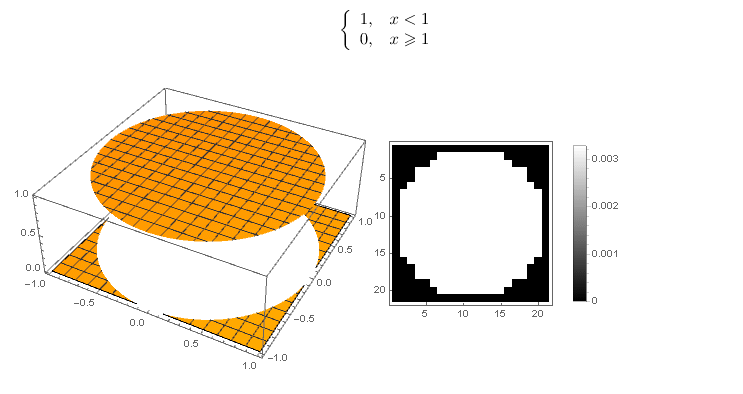
\includegraphics[scale=0.5]{pic1.png}
            \caption*{Источник картинки https://habr.com/ru/post/432622/}
        \end{figure}
 
        При использовании такого (или похожего фильтра) будет получаться данный по условию эффект размытия (с потерей оттенков цветов кожи, теней и т.д.)
        Для решения этой проблемы можно, например добавить зависимость затухания от координаты. Т.е. некоторые участки кожи будут казаться темнее или светлее. Один из таких алгоритмов: размытие по Гауссу.
        
    \end{enumerate}
\end{document}